\documentclass[border=4pt]{standalone}
\usepackage{fontspec}
\usepackage{amsmath}
\usepackage{unicode-math}
\setmainfont{Latin Modern Roman}
\setmathfont{Latin Modern Math}
\usepackage{pgfplots}
\usepackage{pgfplotstable}
\pgfplotsset{compat=1.18}
\usepackage{tkz-euclide}
\usetikzlibrary{arrows.meta,calc,angles,quotes,patterns,3d,backgrounds}
\definecolor{ink}{HTML}{123428}
\definecolor{asy}{HTML}{475569}
\definecolor{mint}{HTML}{86e0bd}
\tikzset{asym/.style={asy, line width=0.9pt, dash pattern=on 5pt off 3.5pt},
         guide/.style={gray!70, line width=0.6pt, densely dotted},
         dot/.style={circle, inner sep=0pt, minimum size=5pt, draw=white, line width=0.5pt},
         odot/.style={circle, inner sep=0pt, minimum size=5.5pt, fill=white, line width=1pt},
         lab/.style={font=\footnotesize, inner sep=1.5pt, text=ink}}
\begin{document}
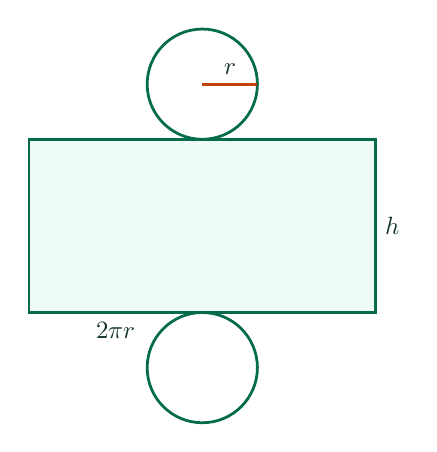
\begin{tikzpicture}
\draw[color={rgb,255:red,4;green,107;blue,77}, line width=1pt, fill={rgb,255:red,134;green,224;blue,189}, fill opacity=0.15] (0,0) rectangle (4.4,2.2);
\draw[color={rgb,255:red,4;green,107;blue,77}, line width=1pt] (2.2,2.9) circle (0.7); \draw[color={rgb,255:red,4;green,107;blue,77}, line width=1pt] (2.2,-0.7) circle (0.7);
\node[font=\small, text=ink, below] at (1.1,0) {$2\pi r$}; \node[font=\small, text=ink, right] at (4.4,1.1) {$h$};
\draw[color={rgb,255:red,194;green,65;blue,12}, line width=1pt] (2.2,2.9) -- (2.9,2.9); \node[font=\small, text=ink, above] at (2.55,2.9) {$r$};
\end{tikzpicture}
\end{document}
